\chapter{Introduction}

Ultra Low Power Processors, such as ARM's Cortex-M0+, are becomming an increasingly appealing area of research, particularly because they provide a platform for the Internet of Things. As our culture develops new ways for technology to aide our every-day lives, the devices which support these progressions are required to be less and less introdusive, forcing companies to search for new methods of making systems smaller and require lower power. In some cases devices are required to run for months or even years using a single power source.

However, such processors clearly create very tight constraints for potencial developers, as processing power is often limited, leading to the ever-continuing requirement for more efficient and optimised algorithms. As memory usage is also proportional to power consumption, the RAM availaible on such systems is also extremely limiting. As we begin to rely on these systems more and more, these constraints make it a growing challenge to implement systems which are not only useful, but can be relied upon to function when needed.

\section{Project Goals}

ARM is currently investigating the concept of a subthreshold Cortex-M0+, which attempts to push the extremes of these constraints further by providing just 8KB of memory for both program code and data, and running at just a few hundred cycles per second. This project aims to research and develop an algorithm which is capable of running on such a device, to act as a proof of concept that such a processor would be worth while.

The particular algorithm that is to be developed is a way to identify and monitor exercises performed by a human wearer. These are specifically exercises which can be done on aeroplanes to reduce the risk of suffering from Deep Vein Thrombosis, a condition where a blood clot can form in one of the deep veins in the body, most commonly the legs. This can lead to further complications such as pulmonary embolism which is when part of the blood clot moves and blocks a blood vessel in the lungs \cite{NHS2014DVT}. Long-haul flights can increase the risk of getting DVT because of the long periods of time sitting down and not moving which reduces circulation in the legs.

\begin{figure}[h]
  \centering
    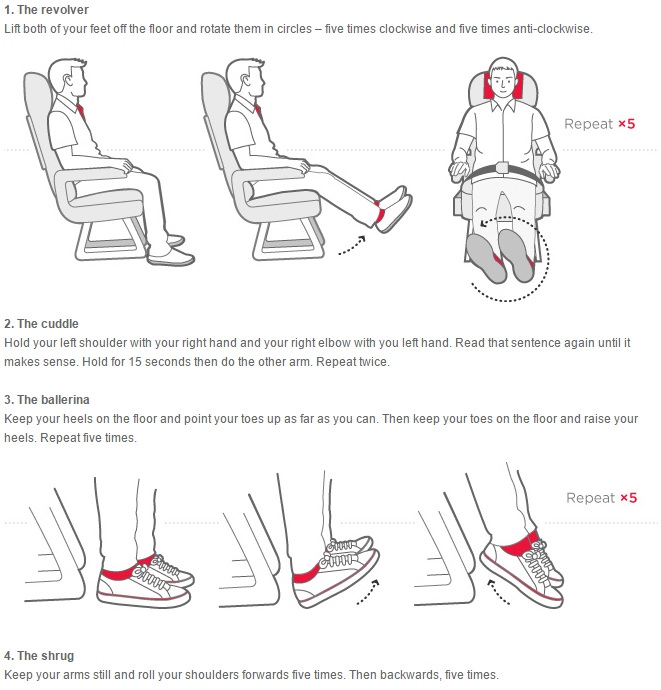
\includegraphics[width=1.0\textwidth]{figures/exercises}
  \caption{Inflight exercises \cite{virgin2015exercises}}
  \label{fig:exercises}
\end{figure}

Figure \ref{fig:exercises} shows some of the inflight exercises which can be performed. We have focussed on a few of them including the revolver, the ballerina and the shrug. These involve rotating the feet in circles, pointing the feet up and down and rolling the shoulders backwards and forwards. These are all designed to help keep the circulation going in the limbs.

Possible uses of the algorithm would be to incorporate it into a device which could be given to passengers to strap to their legs. It would then monitor how much exercise each person was doing. This could help inform the passengers whether or not they are doing enough exercise to stay risk free. The device itself could make use of energy efficient technologies (for example the Cortex-M0+) so that its battery could easily last the entire duration of a long-haul flight.

The project requires us to emulate the proposed subthreshold Cortex-M0+ by creating a test platform that can mimic its processor speed. This is partially because the devivce itself is still in development and as such is not readily available for us to use. A testing platform would also allow us to experiment with different clock speeds when testing the algorithm. The hardware section of this report covers what this involved.

The other substantial aspect of this project is the development of the algorithm itself. Multiple approaches are investigated with a particular focus on machine learning techniques. On top of this, the methods of optimising these techniques to reduce processing and memory demands is also heavily looked at. The trade-offs between resource optimisation and accuracy of the algorithm is also examined.  This part of the project is covered in the software section of the report.

Other parts of the project include a user study to collect movement data of the exercises we are trying to detect. This data is needed in order to develop the algorithm and a user study is an ideal way to collect a range of data from a selection of different people because each individual is likely to perform the exercises with slight variations.

This report concludes by evaluating the final developed algorithm in terms of its accuracy in detecting exercises and its power and resource requirements. This is then used as a basis for determining the suitableness of using constrained subthreshold devices to compute complex problems.


\section{Requirements}

\begin{enumerate}
  \item The algorithm must be capable of detecting and monitoring exercises designed to combat deep vein thrombosis
  \begin{enumerate}[label*=\arabic*.]
    \item These are exercises which can be performed in a plane, particularly in long haul flights and include:
    \begin{enumerate}[label*=\arabic*.]
      \item Foot rotations
      \item Pointing feet up and down
      \item Shoulder rolling
    \end{enumerate}
    \item Other activities such as walking should be distinguished as not being exercise
  \end{enumerate}
  \item The algorithm must be suitable to execute on an ultra-low-power subthreshold ARM Cortex-M0+
  \begin{enumerate}[label*=\arabic*.]
    \item This device has a limited processor clocked from 100 kHz to a maximum of 3 MHz
    \item Memory usage should be kept to a minimum with a target of no more than 8 kB
    \item Therefore, the algorithm should be highly optimised to use as little memory and require as little processing power as possible
  \end{enumerate}
  \item The Cortex-M0+ must be emulated in a test platform as working with an actual M0+ is not feasible
  \begin{enumerate}[label*=\arabic*.]
    \item The test platform should be capable of being clocked at frequencies ranging from a 100s of kHz to a few MHz
    \item The test platform should have at least 32 kB of memory to aid with testing and to act as a fall back if 8 kB cannot be achieved
    \item There must be an accelerometer sensor on the platform that readings can be taken from
  \end{enumerate}
  \item Research into various potential algorithms must take place
  \begin{enumerate}[label*=\arabic*.]
    \item Machine learning approaches should be focussed on
    \item Algorithms which are used on unconstrained systems should be considered first
    \item The feasibility of constraining those algorithms should then be investigated
  \end{enumerate}
  \item Participant studies should be performed to gather movement data to train the algorithm
  \begin{enumerate}[label*=\arabic*.]
    \item Ethics approval will need to be obtained
  \end{enumerate}
  \item The developed algorithm must be deployed to the test platform
  \item The final system must then be evaluated in terms of its accuracy at detecting exercises
\end{enumerate}